\section{Frequency analysis}
\label{sec:analysis}

In this following section an analysis will be made of the sound made by a car motor (figure \ref{fig:car}), windmill (figure \ref{fig:windmill}), EKG, breaking wine glass and four different genres of music. 
The approach of this analysis will be to plot the signal in the time domain, the fourier transformed signal and then som applied functions described in section \ref{sec:theory}.


\subsection{Car engine}

The original signal from the car engine is seen in figure \ref{fig:car_time}, while the Fourier transformed signal is seen in figure \ref{fig:car_freq}. The following are also Fourier transformed, but have applied smoothing (figure \ref{fig:car_smooth}), zeropadding (figure \ref{fig:car_zero}) and hamming (figure \ref{fig:car_window}). Notice the magnitude difference from the Fourier transformed to the smoothing.

\begin{figure}[htb!]
	\centering
	\subcaptionbox{Time Domain.\label{fig:car_time}}
	{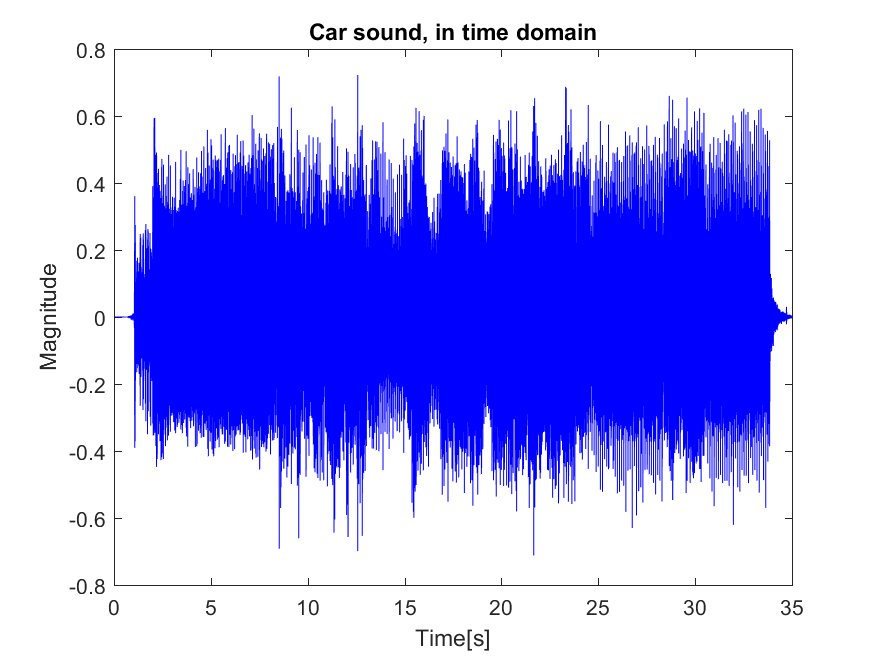
\includegraphics[width=0.45\linewidth]{code/Car_figure1.png}}
	\subcaptionbox{Frequency Domain.\label{fig:car_freq}}
	{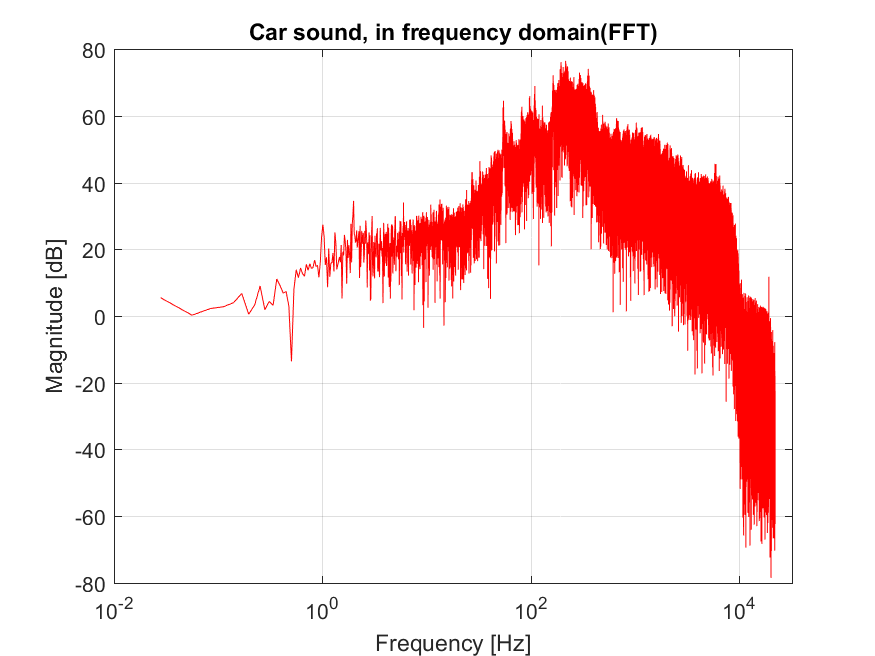
\includegraphics[width=0.45\linewidth]{code/Car_figure2.png}}
	\subcaptionbox{Smoothed fft.\label{fig:car_smooth}}
	{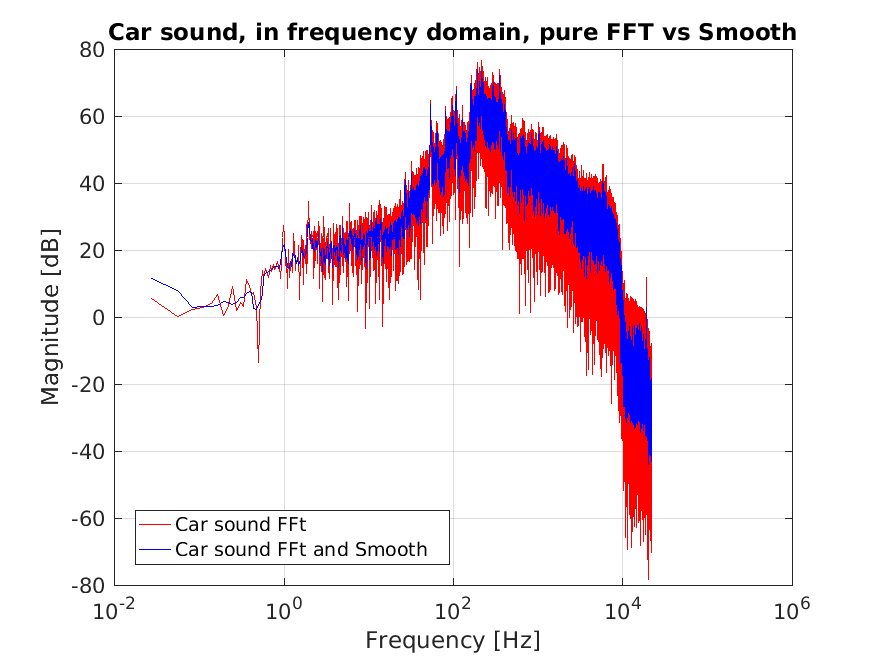
\includegraphics[width=0.45\linewidth]{code/Car_figure3.png}}
	\subcaptionbox{fft of zero padded original.\label{fig:car_zero}}
	{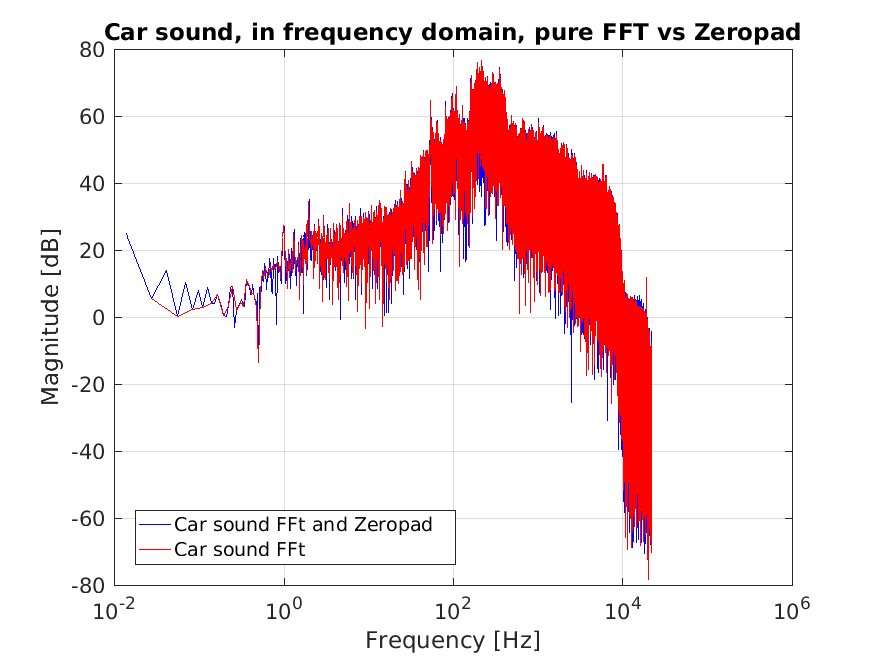
\includegraphics[width=0.45\linewidth]{code/Car_figure4.png}}
	\subcaptionbox{fft of windowed original.\label{fig:car_window}}
	{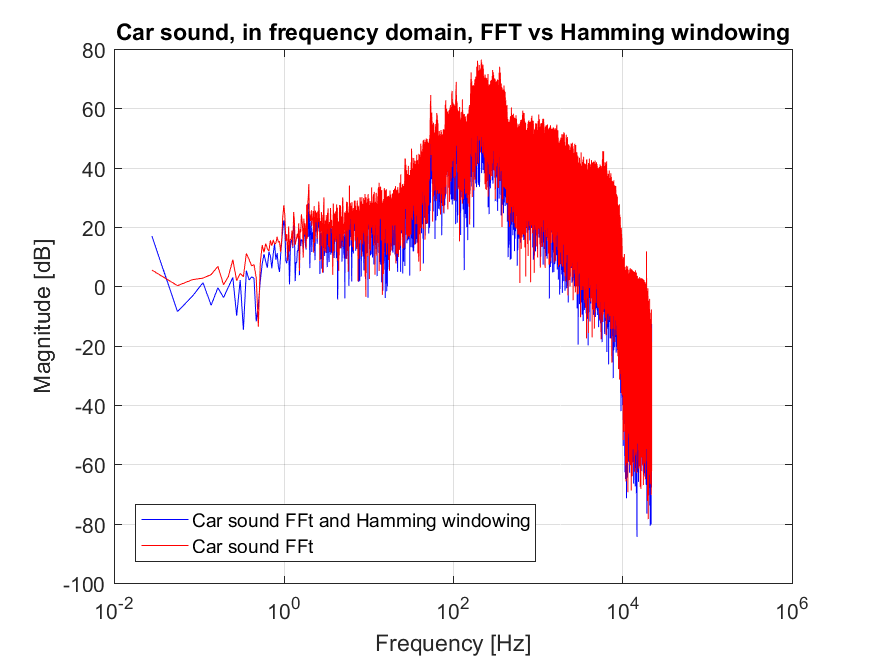
\includegraphics[width=0.45\linewidth]{code/Car_figure5.png}}
	\caption{Analysis of the sound of a car.}\label{fig:car}
\end{figure}

\subsection{Noise from a Windmill}

The original signal from the windmill is seen plotted in the timedomain in figure \ref{fig:windmill_time}, while the fourier transformed signal is seen in figure \ref{fig:windmill_freq}. The following has first applied some function and then is fourier transformed, the smooth function is seen on figure \ref{fig:windmill_smooth}, the zeropadding is seen in figure \ref{fig:windmill_zero} and the window function is seen in figure \ref{fig:windmill_window}.

\begin{figure}[htb!]
	\centering
	\subcaptionbox{Time Domain.\label{fig:windmill_time}}
	{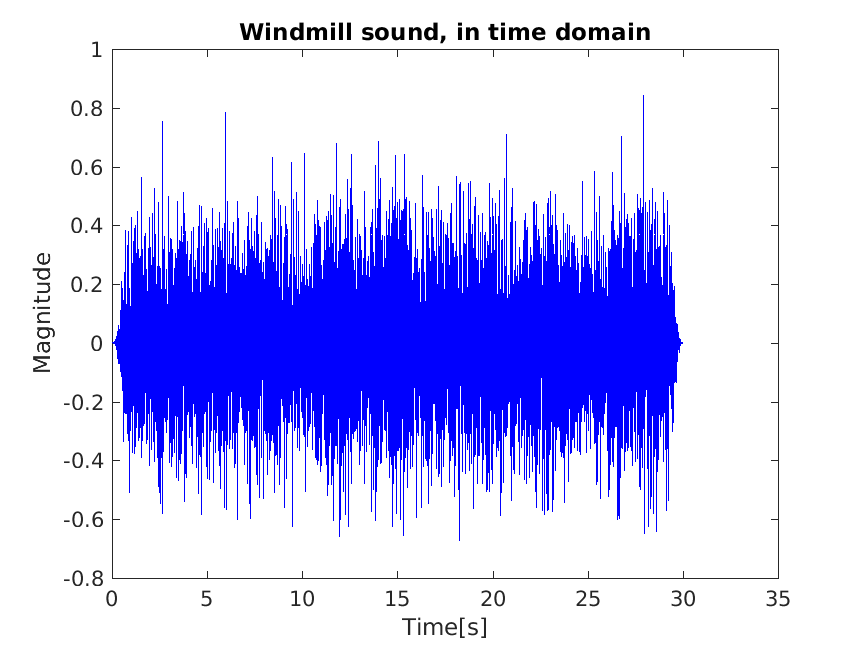
\includegraphics[width=0.45\linewidth]{code/Windmill_figure1.png}}
	\subcaptionbox{Frequency Domain.\label{fig:windmill_freq}}
	{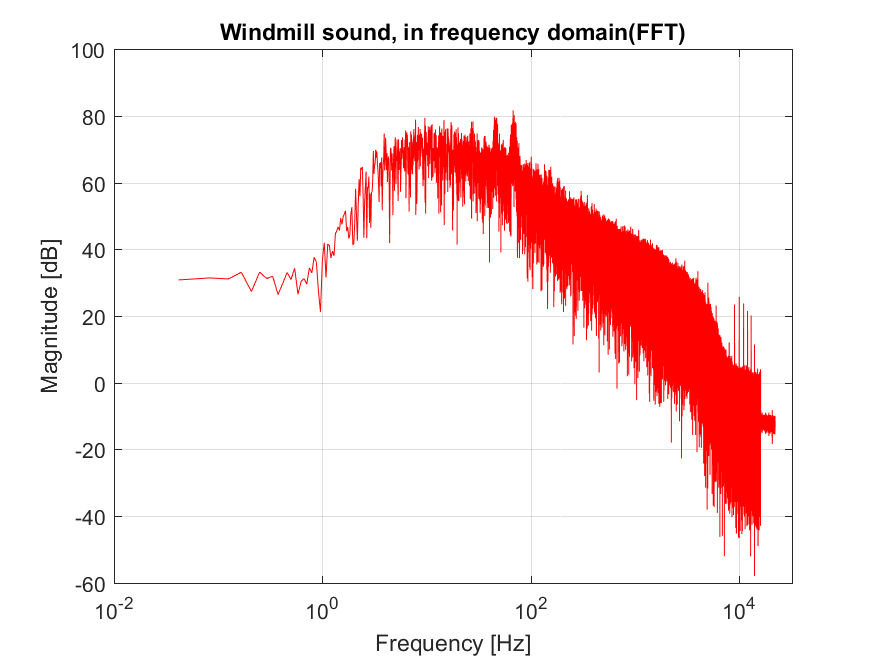
\includegraphics[width=0.45\linewidth]{code/Windmill_figure2.png}}
	\subcaptionbox{Smoothed fft.\label{fig:windmill_smooth}}
	{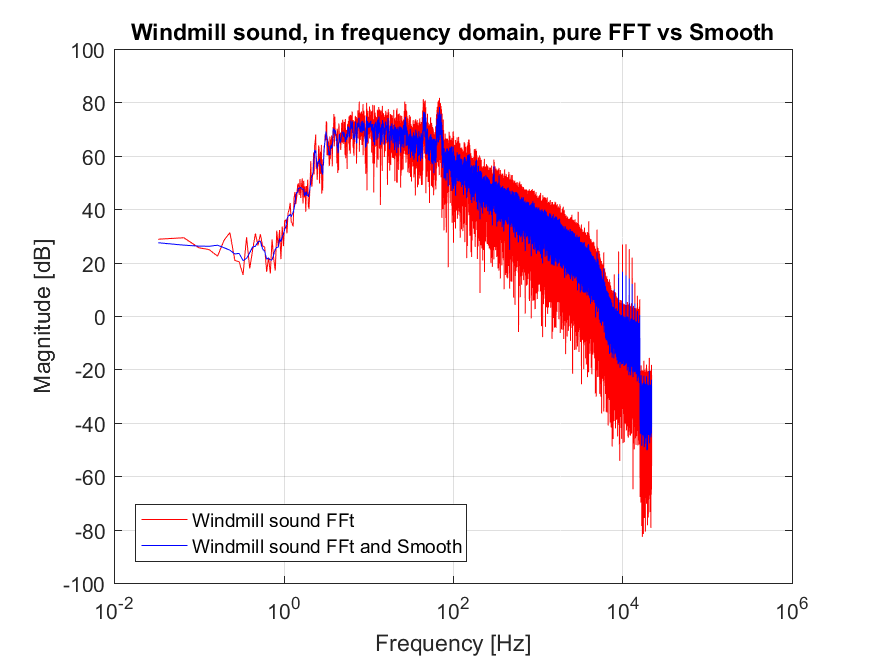
\includegraphics[width=0.45\linewidth]{code/Windmill_figure3.png}}
	\subcaptionbox{fft of zero padded original.\label{fig:windmill_zero}}
	{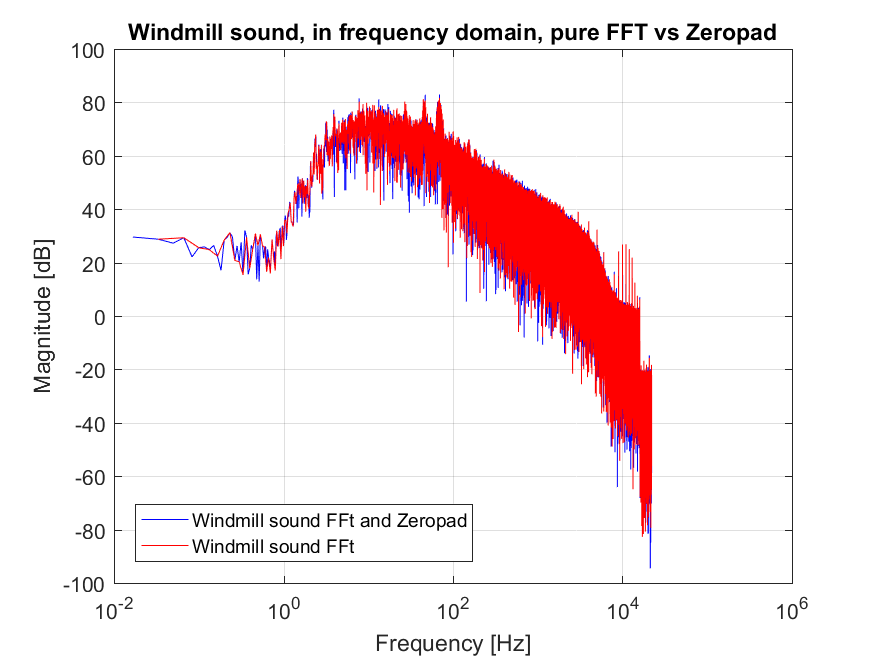
\includegraphics[width=0.45\linewidth]{code/Windmill_figure4.png}}
	\subcaptionbox{fft of windowed original.\label{fig:windmill_window}}
	{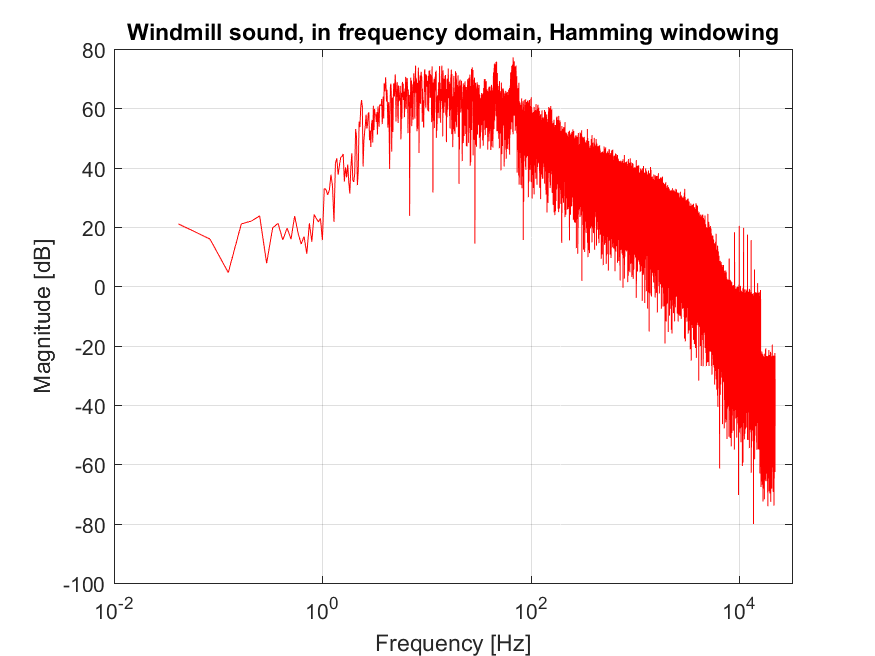
\includegraphics[width=0.45\linewidth]{code/Windmill_figure5.png}}
	\caption{Analysis of the sound of a windmill.}\label{fig:windmill}
\end{figure}


\subsection{EKG}

The original signal from the EKG is seen plotted in the timedomain in figure \ref{fig:ekg_time}, while the fourier transformed signal is seen in figure \ref{fig:ekg_freq}. The following has first applied some function and then is fourier transformed, the smooth function is seen on figure \ref{fig:ekg_smooth}, the zeropadding is seen in figure \ref{fig:ekg_zero} and the window function is seen in figure \ref{fig:ekg_window}.


\begin{figure}[htb]
	\centering
	\subcaptionbox{Time Domain.\label{fig:ekg_time}}
	{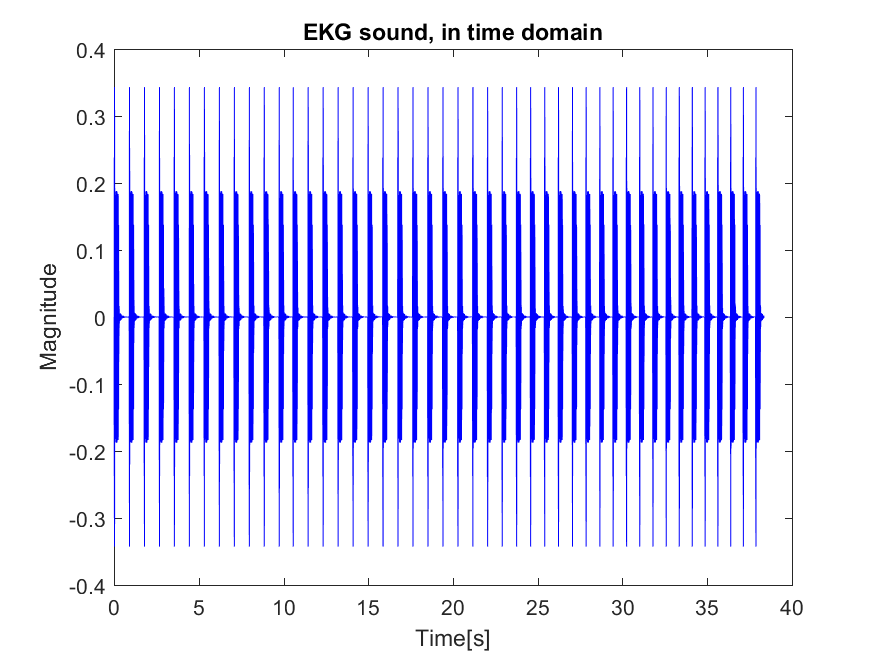
\includegraphics[width=0.45\linewidth]{code/ekg_figure1.png}}
	\subcaptionbox{Frequency Domain.\label{fig:ekg_freq}}
	{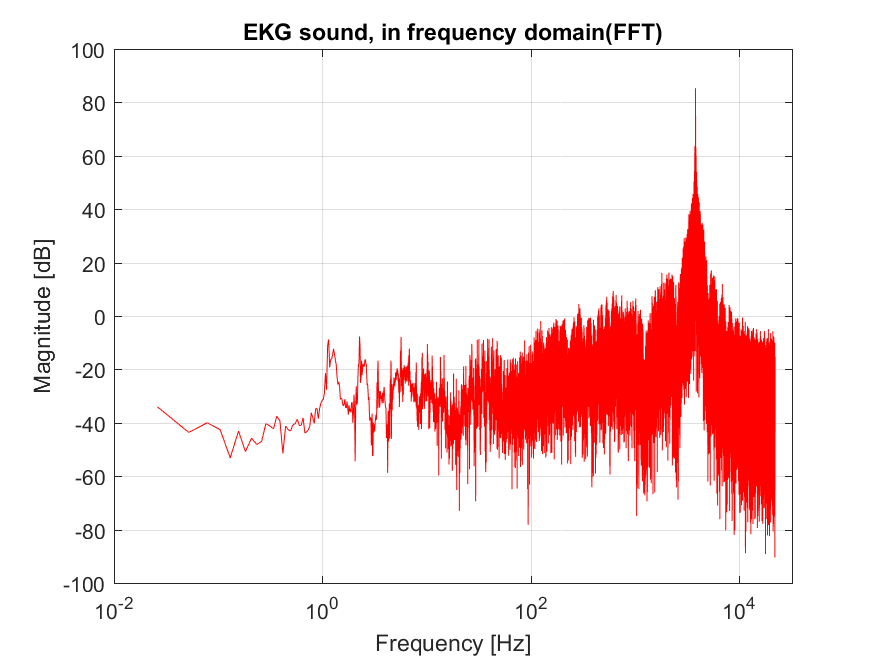
\includegraphics[width=0.45\linewidth]{code/ekg_figure2.png}}
	\subcaptionbox{Smoothed fft.\label{fig:ekg_smooth}}
	{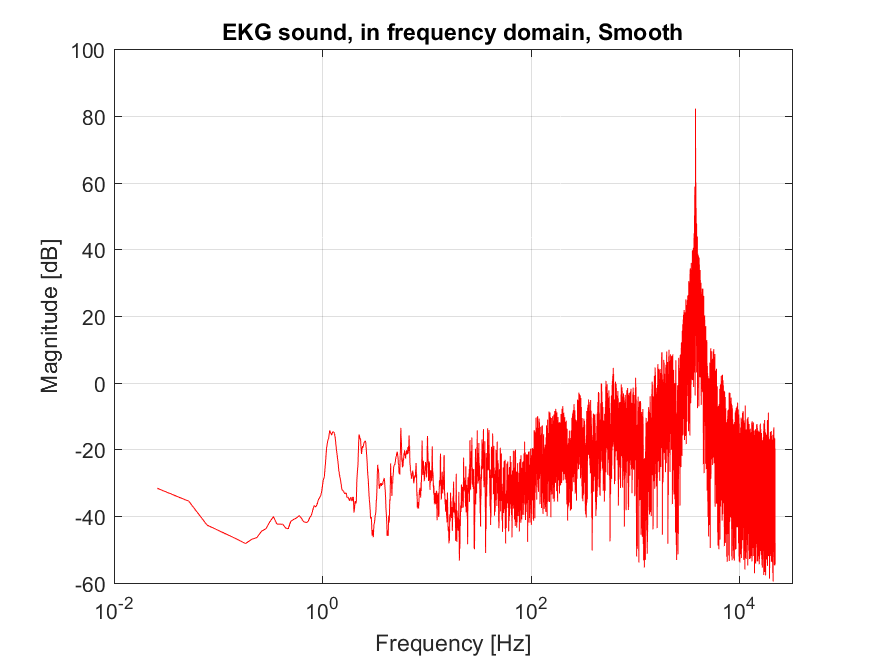
\includegraphics[width=0.45\linewidth]{code/ekg_figure3.png}}
	\subcaptionbox{fft of zero padded original.\label{fig:ekg_zero}}
	{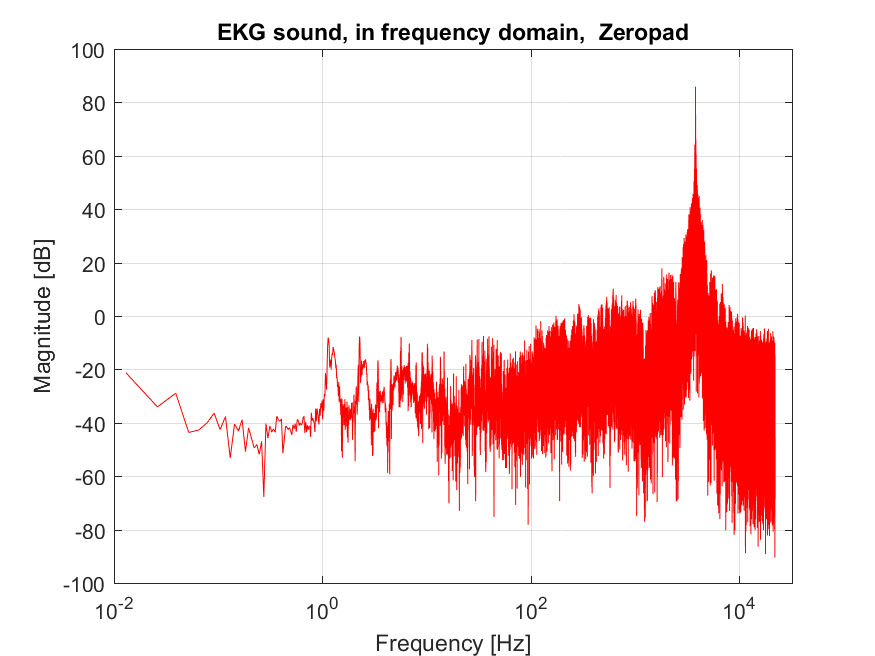
\includegraphics[width=0.45\linewidth]{code/ekg_figure4.png}}
	\subcaptionbox{fft of windowed original.\label{fig:ekg_window}}
	{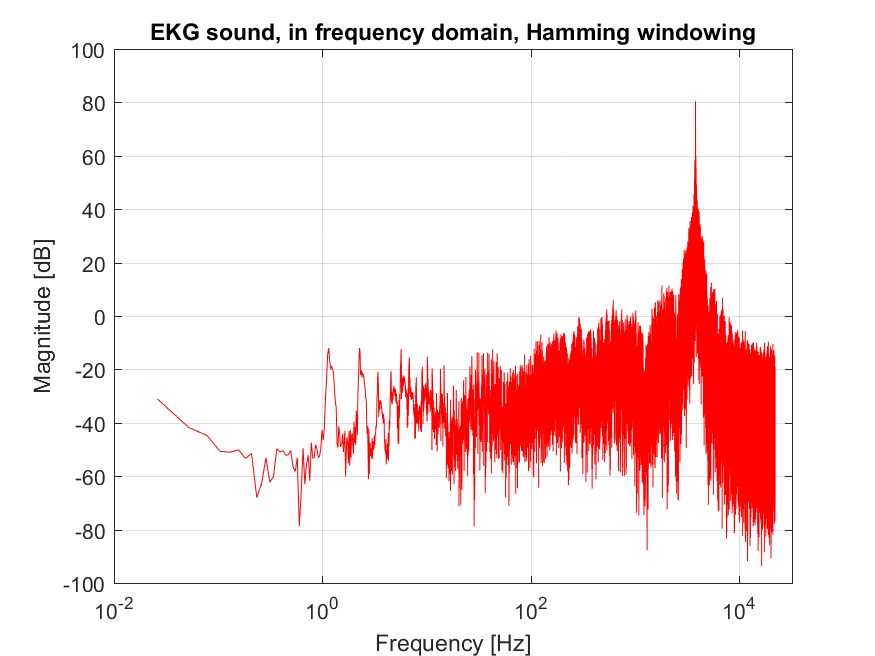
\includegraphics[width=0.45\linewidth]{code/ekg_figure5.png}}
	\caption{Analysis of the sound of an EKG.}\label{fig:ekg}
\end{figure}

\subsection{Breaking Wine Glass}

\begin{figure}[htb]
	\centering
	\subcaptionbox{Time Domain.\label{fig:glassBreaking_time}}
	{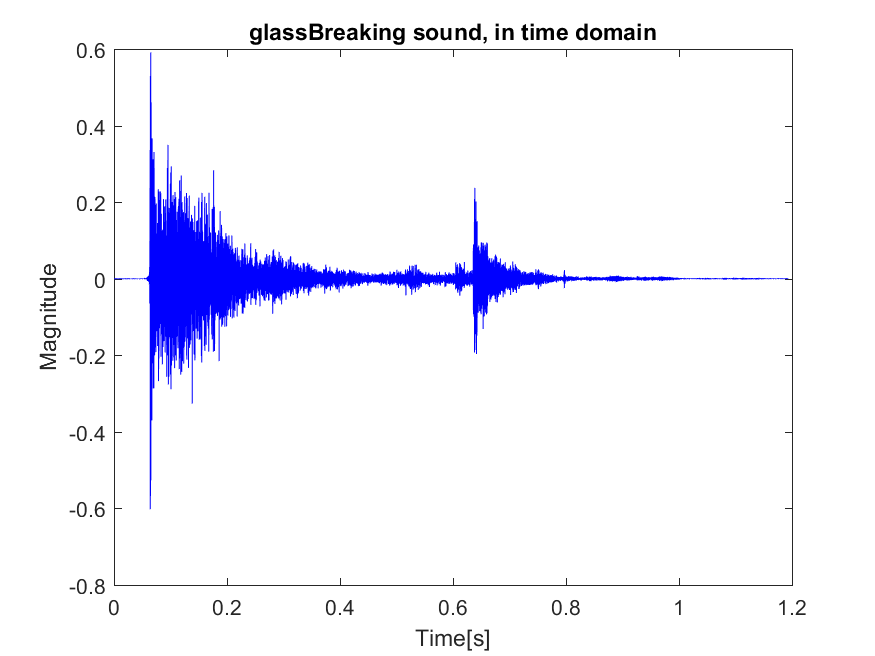
\includegraphics[width=0.45\linewidth]{code/glassBreaking_figure1.png}}
	\subcaptionbox{Frequency Domain.\label{fig:glassBreaking_freq}}
	{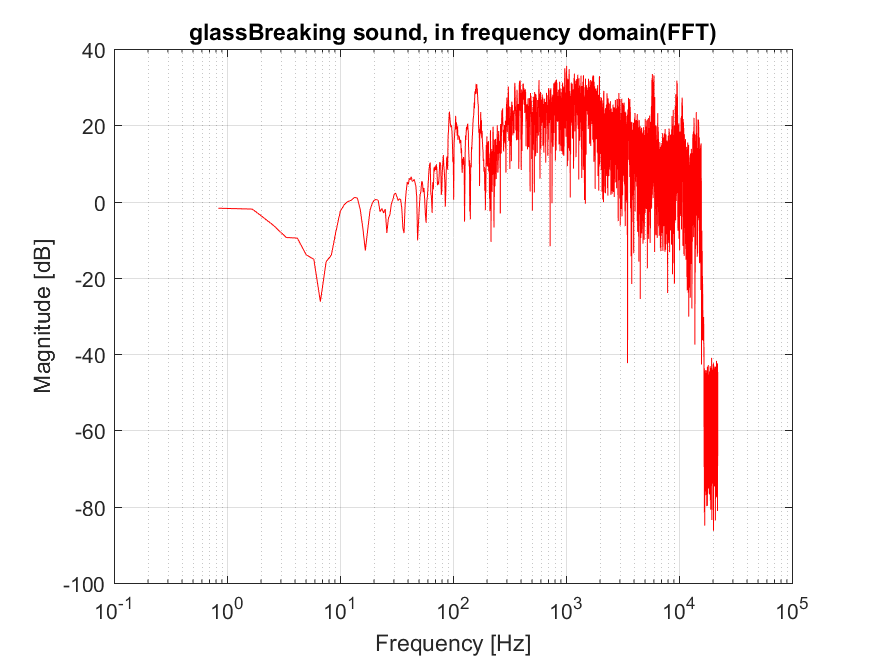
\includegraphics[width=0.45\linewidth]{code/glassBreaking_figure2.png}}
	\subcaptionbox{Smoothed fft.\label{fig:glassBreaking_smooth}}
	{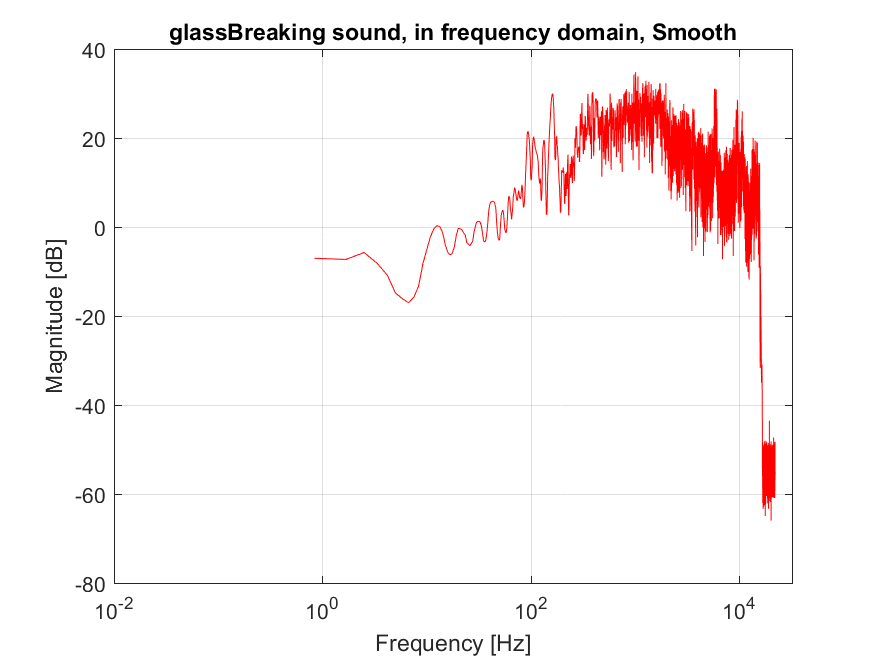
\includegraphics[width=0.45\linewidth]{code/glassBreaking_figure3.png}}
	\subcaptionbox{fft of zero padded original.\label{fig:glassBreaking_zero}}
	{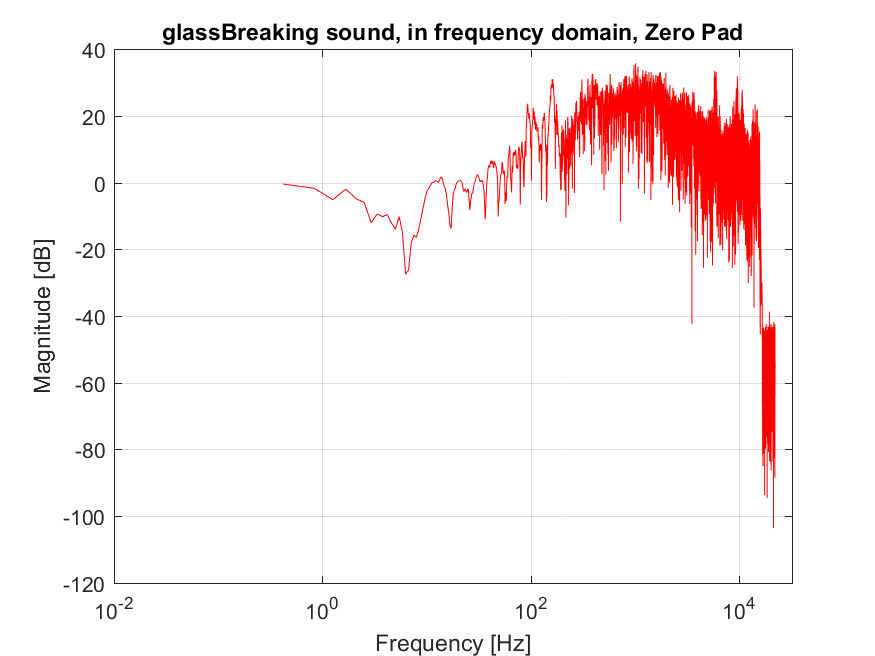
\includegraphics[width=0.45\linewidth]{code/glassBreaking_figure4.png}}
	\subcaptionbox{fft of windowed original.\label{fig:glassBreaking_window}}
	{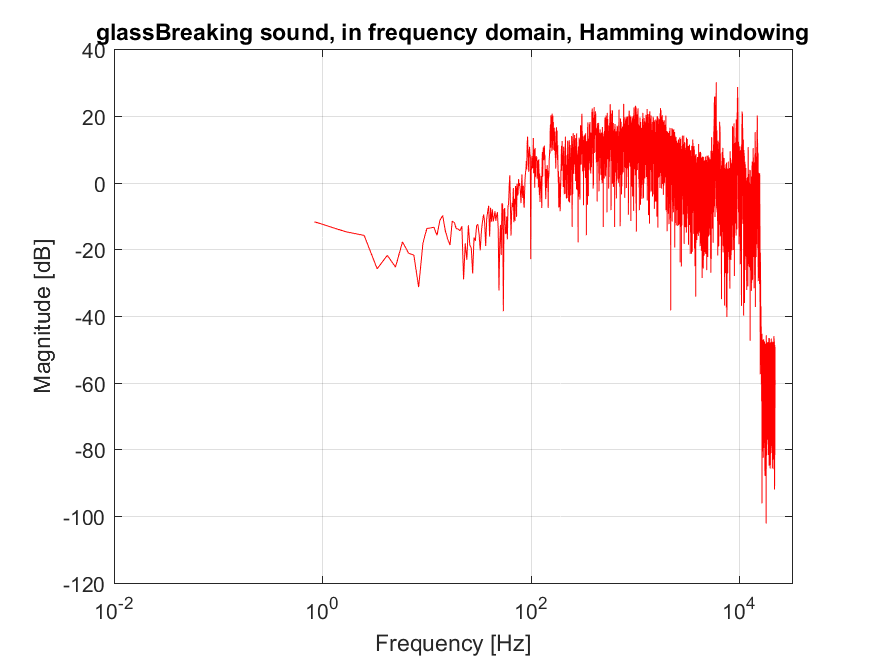
\includegraphics[width=0.45\linewidth]{code/glassBreaking_figure5.png}}
	\caption{Analysis of the sound of a glas breaking.}\label{fig:glassBreaking}
\end{figure}


\subsection{Music}

\paragraph{Pop}
Michael Jackson - Thriller

\begin{figure}[htb]
	\centering
	\subcaptionbox{Time Domain.\label{fig:pop_time}}
	{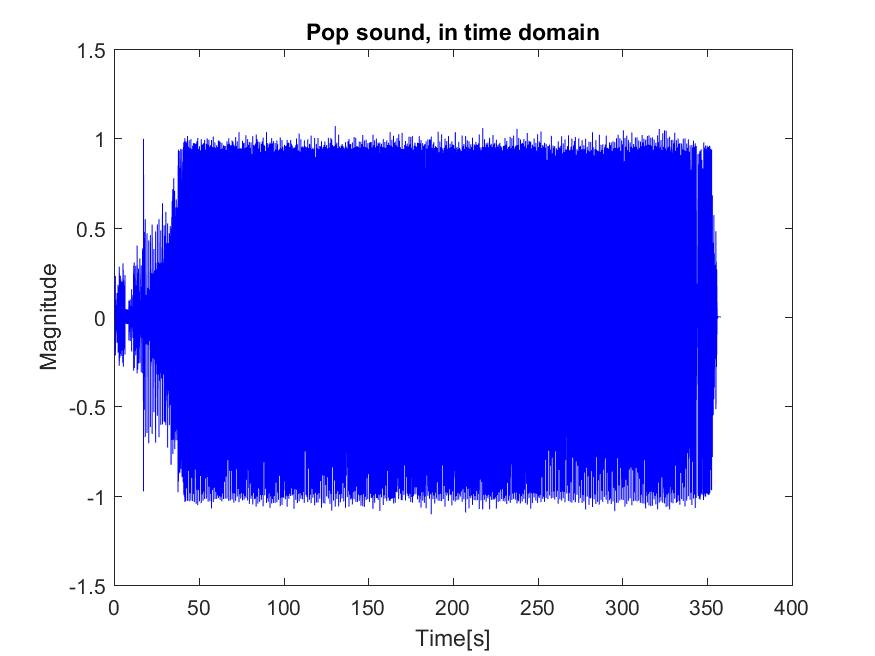
\includegraphics[width=0.45\linewidth]{code/Pop_figure1.png}}
	\subcaptionbox{Frequency Domain.\label{fig:pop_freq}}
	{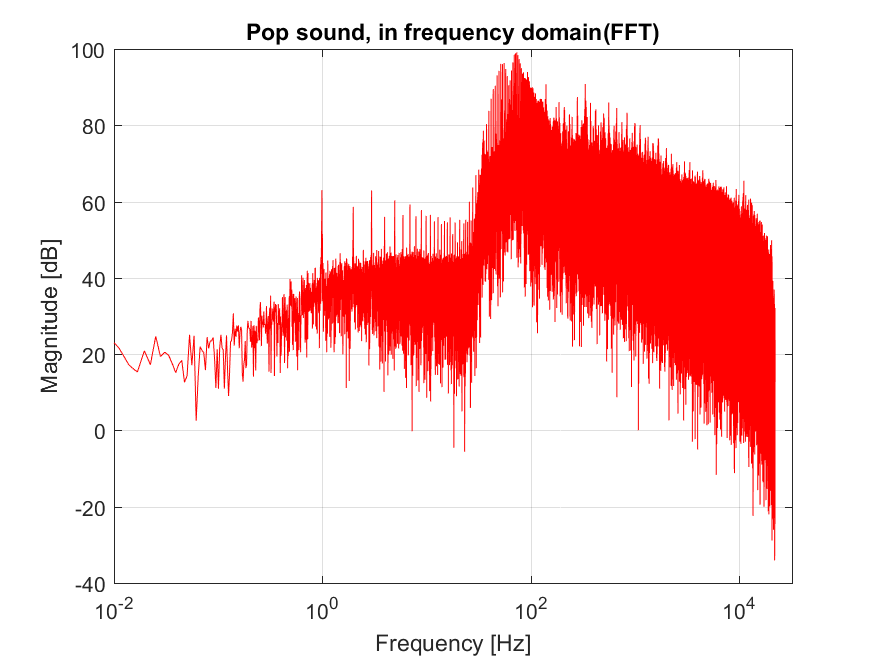
\includegraphics[width=0.45\linewidth]{code/Pop_figure2.png}}
	\subcaptionbox{Smoothed fft.\label{fig:pop_smooth}}
	{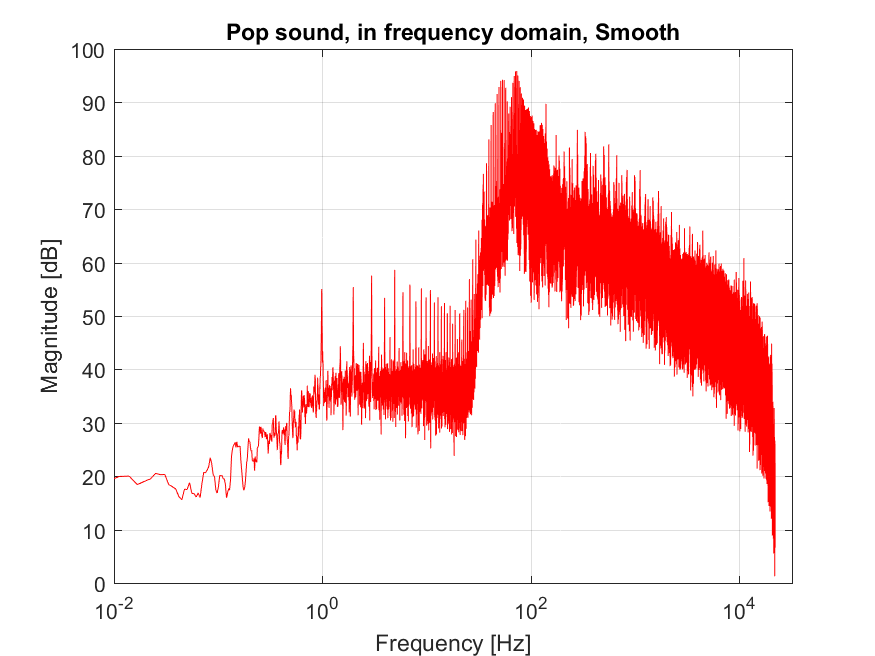
\includegraphics[width=0.45\linewidth]{code/Pop_figure3.png}}
	\subcaptionbox{fft of zero padded original.\label{fig:pop_zero}}
	{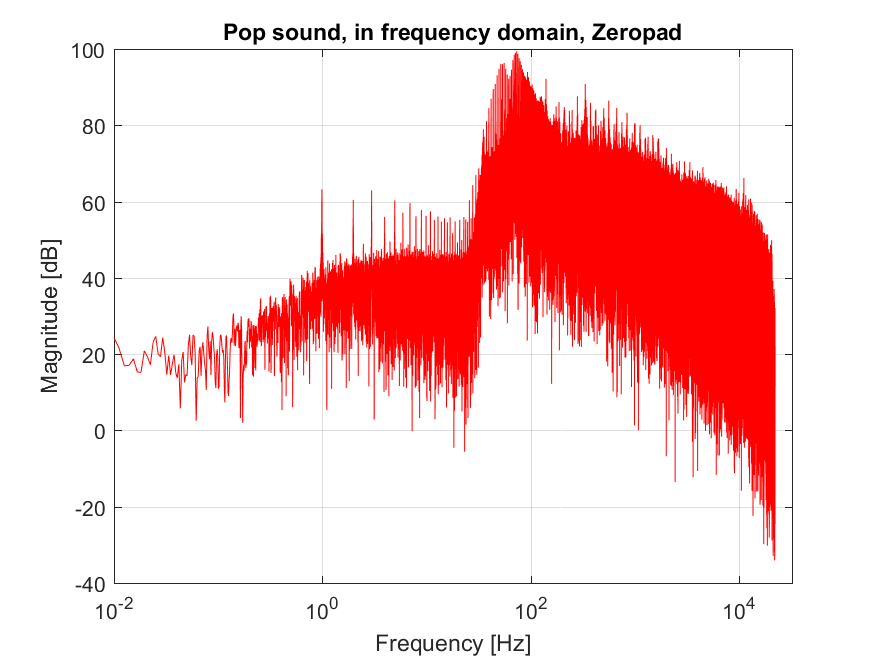
\includegraphics[width=0.45\linewidth]{code/Pop_figure4.png}}
	\subcaptionbox{fft of windowed original.\label{fig:pop_window}}
	{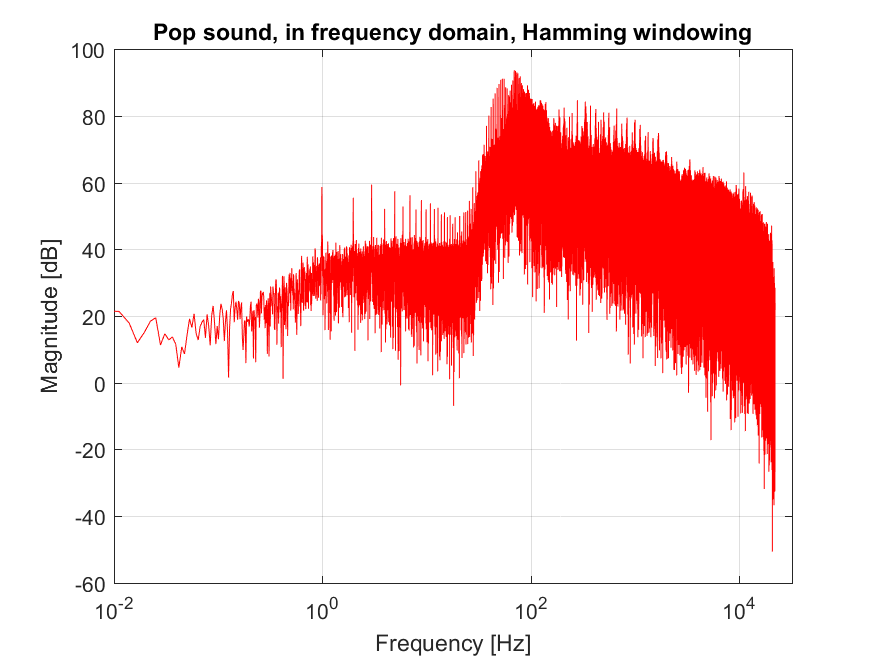
\includegraphics[width=0.45\linewidth]{code/Pop_figure5.png}}
	\caption{Analysis of the sound of Pop.}\label{fig:pop}
\end{figure}

\paragraph{Tekno}
Matador - The Enemy ft Felix Da Housecat (Original Mix)

\begin{figure}[htb]
	\centering
	\subcaptionbox{Time Domain.\label{fig:techno_time}}
	{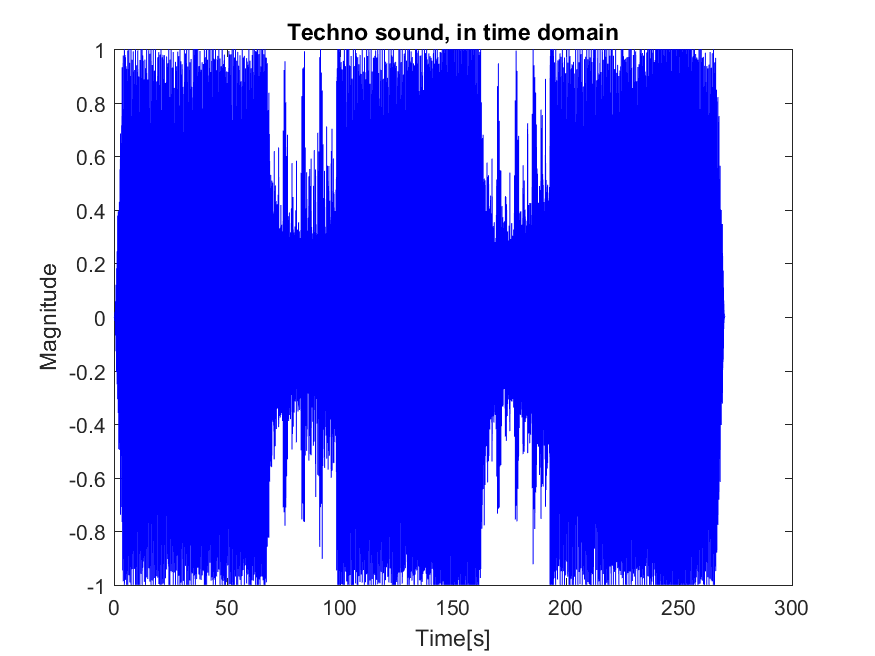
\includegraphics[width=0.45\linewidth]{code/Techno_figure1.png}}
	\subcaptionbox{Frequency Domain.\label{fig:techno_freq}}
	{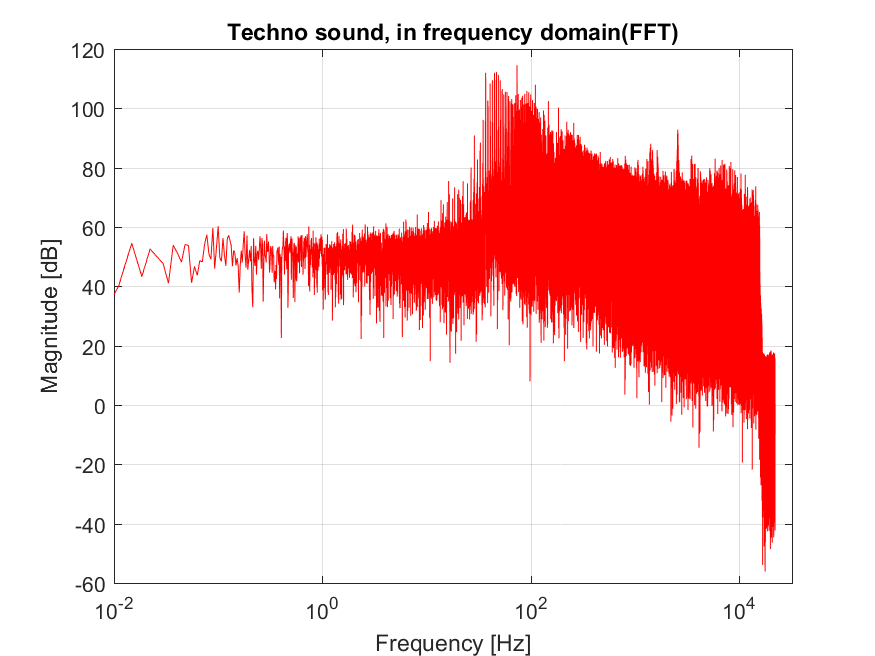
\includegraphics[width=0.45\linewidth]{code/Techno_figure2.png}}
	\subcaptionbox{Smoothed fft.\label{fig:techno_smooth}}
	{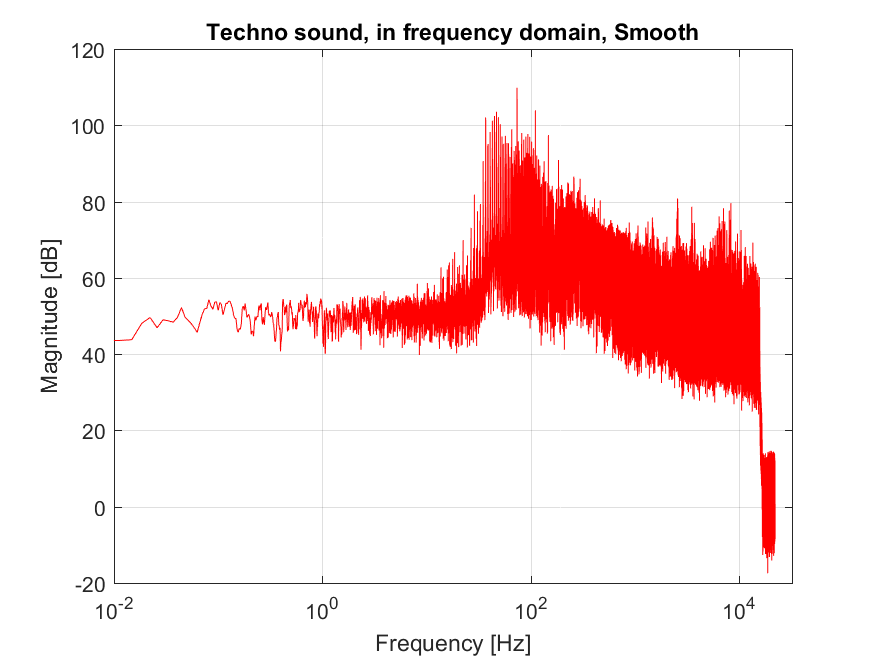
\includegraphics[width=0.45\linewidth]{code/Techno_figure3.png}}
	\subcaptionbox{fft of zero padded original.\label{fig:techno_zero}}
	{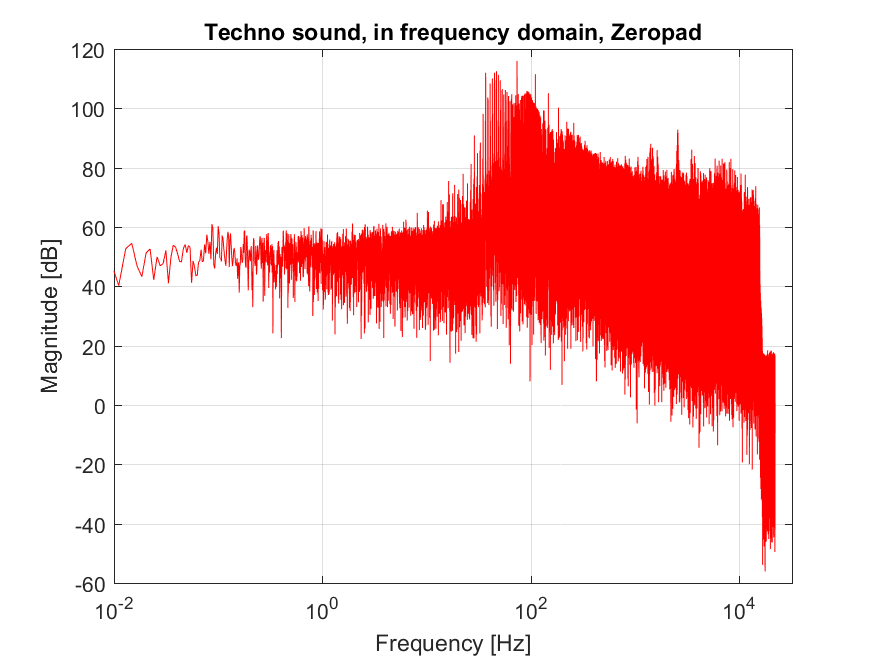
\includegraphics[width=0.45\linewidth]{code/Techno_figure4.png}}
	\subcaptionbox{fft of windowed original.\label{fig:techno_window}}
	{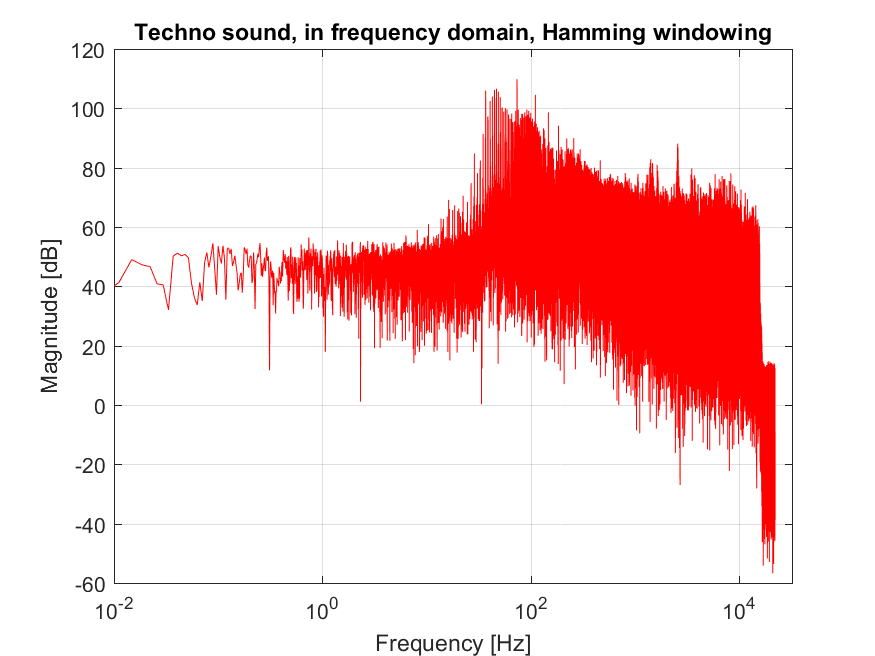
\includegraphics[width=0.45\linewidth]{code/Techno_figure5.png}}
	\caption{Analysis of the sound of Techno.}\label{fig:techno}
\end{figure}

\paragraph{Heavy Metal}

\paragraph{Klassisk}

\subsubsection{Conclusion}


\section{Energy} 
\Cref{tab:Energy} shows the energies in signals before and after the Fourier transform. It clearly shows that there is no loss of energy between the original signal and a Fourier transform, but when smoothing and windowing is applied there is a potential loss of energy.
While zero padding does not add or remove any energy from the signal.
\begin{table}[htb!]
	\centering
	\begin{tabularx}{\textwidth}{p{2cm} | X X X X X}
		& \rotatebox{90}{\textbf{Time Domain $\times\num{e4}$}}   & \rotatebox{90}{\textbf{Frequency Domain $\times\num{e4}$}} & \rotatebox{90}{\textbf{Smooth $\times\num{e3}$}}     & \rotatebox{90}{\textbf{Zero Padding $\times\num{e4}$}}  & \rotatebox{90}{\textbf{Windowing $\times\num{e4}$}} \\
		\hline
		Car Engine  & \num{3,07}	& \num{3,07}	& \num{0,686}  &	\num{3,07}  & \num{1,34}  \\
		
		Windmill	& \num{4,14}	& \num{4,14}	& \num{0,521} & \num{4,14} & \num{1,79} \\
		
		Breaking Wine Glass & \num{0,0115}	& \num{0,0115}	& \num{0,155}	& \num{0,0115}	& \num{0,000265} \\
		
		EKG & \num{2,05}	& \num{2,05}	& \num{0,626}	& \num{2,05}	& \num{0,729} \\
		
		Pop & & & & & \\
		
		Electronica & & & & & \\
		
		Heavy Metal & & & & & \\
		
		Klassisk & & & & & \\
	\end{tabularx}
	
	\caption{Energy of the different signals shown in \si{\joule}.}
	\label{tab:Energy}
\end{table}

Eksperimenter med udglatning, zero-padding og windowing 